\section{Exterior extensions: the March proposal and its precise replacement}
\label{ext:section}

The starting point of this project was the March 2026 proposal that an odd
Kobon arrangement could always be extended with the gain
\begin{equation}
  \K(2m+2)\geq \K(2m+1)+m.
  \label{ext:march}
\end{equation}
The proposal was presented in \cite{zarzuelo2026} and subsequently described
as an iterative rule in \cite{handwiki2026}.  The preserved March source is
important evidence of the development of the idea, but is not a completed
proof of \eqref{ext:march}: its Lean file contains eight proof placeholders,
including the extension assertion.  The present work replaces the informal
alternating-segment argument by an actual geometric extension theorem and
identifies exactly which additional counting hypothesis yields the desired
gain.  Independently verified finite bounds are retained regardless of the
status of that original argument.

The later OEIS attribution at orders 28, 30, and 34 is evidence of the
proposal's reception, rather than a proof of numerical
priority~\cite{oeisA006066}.  In particular, the BBL table already records
the straight-line value $30:275$.  The perfect 33-line input belongs to
the family of Forge and Ram\'irez Alfons\'in~\cite{forge1998}; applying the
exterior extension stated by BBL gives $34:357$~\cite{bbl2008}.
The historical attribution, the validity of a finite count, and the
novelty of a general extension theorem are therefore assessed separately.

Two distinctions are essential.  A recurrence for maxima need not extend
\emph{every} arrangement attaining a given count, and a construction for one
odd-to-even step need not admit repeated full-gain extensions.  Throughout
this section the geometric hypotheses concern simple affine arrangements;
consequently their conclusions give lower bounds for both $\Ks$ and $\K$,
but nonsimple witnesses for $\K$ cannot automatically be substituted into
the hypotheses.

\subsection{A geometric theorem from explicitly visible pairs}

Write an old line as $L_i=\{p:\ell_i(p)=0\}$, with $\ell_i$ affine, and let
$A=\{L_0,\ldots,L_{n-1}\}$ be simple.  A linear functional $w$ is
\emph{admissible} if it is nonzero on every old line direction.  At
$p_{ij}=L_i\cap L_j$, choose the direction vectors $u_i,u_j$ on the two
supports so that $w(u_i)=w(u_j)=1$.  The following criterion uses only the
old arrangement.

\begin{definition}[Visible pair]
\label{ext:visible}
The pair $\{i,j\}$ is visible from $w$ if, for every old affine equation
$\ell_k$, the three real numbers
\[
  \ell_k(p_{ij}),\qquad D\ell_k(u_i),\qquad D\ell_k(u_j)
\]
have one common weak sign: either all are nonnegative or all are
nonpositive.  Here $D\ell_k$ denotes the linear part of $\ell_k$.
\end{definition}

Geometrically, the two increasing-$w$ rays bound an unbounded empty wedge.
The algebraic definition is convenient because it gives the required
half-plane inequalities directly, without assuming that a future triangle
already exists.

\begin{theorem}[Verified exterior realization]
\label{ext:realization}
Let $A$ be a simple arrangement of $n$ real affine lines, let $\mathcal T$
be a set of $T$ distinct triangular cells of $A$, and let $\mathcal V$ be
a set of $c$ distinct pairs visible from an admissible $w$.  If
\[
  H>\max_{i<j}w(p_{ij}),
\]
then adjoining $L=\{p:w(p)=H\}$ produces a simple arrangement containing
all triangles in $\mathcal T$ and at least $c$ further triangles.  In
particular, $\Ks(n+1)\geq T+c$.
\end{theorem}

\begin{proof}
Admissibility excludes a parallel old line, and the strict height
inequality excludes every old vertex from $L$.  Thus simplicity is
preserved.  Every old triangle lies in the convex hull of its vertices,
strictly below the level $H$, and survives unchanged.

For a visible pair, the new vertices on its two supports are
\[
 p_{ij}+(H-w(p_{ij}))u_i,
 \qquad p_{ij}+(H-w(p_{ij}))u_j.
\]
At either vertex an old affine equation has the form
\[
 \ell_k(p_{ij})+(H-w(p_{ij}))D\ell_k(u).
\]
The second coefficient is positive.  Definition~\ref{ext:visible}
therefore puts all three vertices in one closed half-plane of each old
line.  The new line is itself a supporting side, and the triangle is
nondegenerate because the old intersection lies strictly below it.  No
arrangement line cuts its interior.  Different old pairs give different
support triples, and every new triple uses $L$, whereas no old one does.
The two lists are consequently disjoint.
\end{proof}

This is the geometric content of \texttt{Exterior.extension}.  The theorem
is proved for arbitrary real coefficients and either parity, with no
assumption about a future triangle count.  An explicit formal height is
\[
  H=1+\sum_{\substack{i,j<n\\i\ne j}}|w(p_{ij})|,
\]
so existence of a sufficiently distant line is part of the construction.
The proof uses the standard Lean logical axioms and no finite native
evaluation.  What it does \emph{not} supply is a universal lower bound of
$\lfloor n/2\rfloor$ on the number of visible pairs.

\subsection{Defect, boundary wedges, and a rule for both parities}

Let $t(A)=T$ and define the bounded-segment defect
\begin{equation}
 d(A)=n(n-2)-3T.
 \label{ext:defect}
\end{equation}
There are $n(n-2)$ elementary bounded segments.  A segment can support at
most one triangular cell: its endpoints determine the two other supports,
and their intersection lies on at most one side of the segment.  Thus
$d(A)$ counts the unused bounded segments.  Let $b(A)$ count the unbounded
two-sided cells, called wedges below.

\begin{lemma}[Boundary charging]
\label{ext:charging}
For a simple arrangement of $n\geq3$ lines,
\[
  3\leq b(A)\leq n,\qquad b(A)+d(A)\geq n.
\]
\end{lemma}

\begin{proof}
The arrangement has $2n$ free rays.  A wedge pairs two such rays at their
common endpoint, and each free ray belongs to at most one wedge.  An
unpaired ray on $L$, ending at $p=L\cap M$, meets an interior vertex of
$M$.  The two bounded elementary segments of $M$ incident to $p$ cannot
both support triangles: both triangles would also use the unique bounded
segment of $L$ starting at $p$.  Charge the unpaired ray to an unused
segment of $M$ at $p$.  Each unused segment receives at most two charges,
one at each endpoint.  Hence $2n-2b\leq2d$.  This also proves $b\leq n$.
Finally, the convex hull of all finite vertices has at least three
vertices.  Both supports at a hull vertex have free outgoing rays, which
give a wedge.  Distinct hull vertices give distinct wedges.
\end{proof}

Order the $2n$ oriented line directions cyclically.  The two directions
of a wedge are consecutive: a line direction strictly inside that sector
would force a line to enter the wedge and cross a free boundary ray.
Write $B\subset\mathbb Z/(2n)$ for the wedge-start indices.  Define
\begin{equation}
 c_j=\bigl|B\cap\{j,j+1,\ldots,j+n-2\}\bigr|,
 \qquad C(A)=\max_j c_j.
 \label{ext:profile}
\end{equation}
The $n$ directions on which an admissible $w$ is positive form one
consecutive block, and every such block occurs for some normal sector.
An exterior line closes precisely the wedges whose two rays lie in this
block.  Consequently $C(A)$ is the exact largest exterior gain and
\begin{equation}
 \sum_{j=0}^{2n-1}c_j=(n-1)b(A),\qquad
 \left\lceil\frac{(n-1)b(A)}{2n}\right\rceil
 \leq C(A)\leq\left\lfloor\frac n2\right\rfloor.
 \label{ext:average}
\end{equation}
The sum follows by counting the $n-1$ blocks containing a fixed wedge.
The upper bound follows because complete wedge pairs use disjoint rays
in a block of $n$ rays.

\begin{theorem}[Boundary-defect extension]
\label{ext:defect-theorem}
For a simple $n$-line arrangement with $n\geq3$ and $T$ triangles, an
exterior line preserves the old triangles and gives at least
\begin{equation}
 T+g(n,T),\qquad
 g(n,T)=\left\lceil\frac{n-1}{2n}
       \max\{3,\,3T-n(n-3)\}\right\rceil
 \label{ext:g}
\end{equation}
triangles.  Thus, for either parity,
\[
 \Ks(n)\geq T\quad\Longrightarrow\quad
 \Ks(n+1)\geq T+g(n,T).
\]
\end{theorem}

\begin{proof}
Lemma~\ref{ext:charging} gives
$b(A)\geq\max\{3,n-d(A)\}$.  Substitute into
\eqref{ext:average} and apply Theorem~\ref{ext:realization}.  If $T$ is
only a lower bound, the witness has some count $T'\geq T$; the right side
of \eqref{ext:g} is nondecreasing in $T$, which gives the stated
maximum-function implication.
\end{proof}

\begin{remark}[Formal scope and attribution]
\label{ext:defect-scope}
Theorem~\ref{ext:defect-theorem} is an ordinary geometric theorem in this
manuscript.  The cyclic sum, averaging argument, and defect arithmetic are
Lean checked, and Theorem~\ref{ext:realization} supplies actual geometric
realization.  The universal charging map and the correspondence between
Euclidean boundary rays and the finite cyclic data have not yet been
joined into an end-to-end Lean proof.  Exterior addition and
unused-segment arguments have precedents in
\cite{bbl2008,blanc2011}.  The contribution under investigation is the
explicit quantitative defect formulation and its certificate interface;
first numerical or historical priority is not asserted.
\end{remark}

\begin{corollary}[Full gain for an odd saturated input]
\label{ext:odd-full}
If a simple arrangement of $2m+1$ lines has defect at most two, an exterior
line creates exactly $m$ additional triangles.  In particular, this
applies to every simple odd arrangement attaining
$\lfloor n(n-2)/3\rfloor$.
\end{corollary}

\begin{proof}
The wedge count is at least $2m-1$.  If all $4m+2$ direction sectors had
gain at most $m-1$, then
\[
 2m(2m-1)\leq 2m b(A)=\sum_jc_j
 \leq(4m+2)(m-1)=2m(2m-1)-2,
\]
a contradiction.  Equation~\eqref{ext:average} bounds the gain above by
$m$.  The segment-count upper bound at odd $n$ leaves defect zero or two.
\end{proof}

For an even input $n=2m$, the sufficient condition $b(A)\geq2m-1$ likewise
forces gain $m$, because $(2m-1)^2>4m(m-1)$.  In either parity the exact
criterion is the finite condition $C(A)=\lfloor n/2\rfloor$.
There is no claim that every even or odd maximum has this boundary
profile.  Iterating \eqref{ext:g} is nevertheless legitimate ordinary
geometry and supplies a weaker lower-bound rule from any simple seed.

\subsection{What fails in indefinite full-gain exterior iteration}

The March argument made the number of new triangles follow from an
alternation assertion after placing a line far from all old vertices.
Distance proves preservation; it does not prove emptiness for half the
new segments.  For example, the five lines $y=ix+i^2$, $i=0,\ldots,4$,
have three triangles, and adding $y=x/2+100$ creates only one further
triangle.  These counts are checked by exact certificates.  This refutes
that unqualified step of the argument, without refuting a better choice
of line or an inequality about maxima.

A stronger obstruction concerns every chain of exterior additions.
Write $b_r$ for its wedge count and $c_r$ for the gain at step $r$.
Closing $c_r$ wedges consumes those wedges.  No new free ray can appear
at an old vertex, and a wedge at a new vertex must use one of the two
free rays of the newly added line.  Therefore
\begin{equation}
 b_{r+1}+c_r\leq b_r+2,
 \qquad
 \sum_{j<r}c_j\leq b_0+2r-b_r\leq b_0+2r-3.
 \label{ext:budget}
\end{equation}
The accumulated exterior gain is at most linear in the number of steps.
The accumulated gains $\lfloor n/2\rfloor$ are quadratic, so an infinite
chain of such full-gain exterior steps is impossible.  The numerical
contradiction is formalized in
\texttt{Iteration.no\_infinite\_full\_gain\_budget}; as in
Remark~\ref{ext:defect-scope}, the universal wedge-budget interpretation
is an ordinary geometric argument.

\begin{table}[tb]
\centering
\small
\begin{tabular}{rrrrr}
\hline
Input order & Triangles & Wedges & Best exterior gain & Requested gain\\
\hline
49&767&47&24&24\\
50&791&24&23&25\\
51&814&3&2&25\\
52&816&3&2&26\\
53&818&3&2&26\\
\hline
\end{tabular}
\caption{One exact greedy exterior chain from the attributed 49-line
input.  Every direction sector was counted with rational arithmetic.
These are capacities of the displayed arrangements, not upper bounds
for $\K$ or $\Ks$ at the corresponding orders.}
\label{ext:49-table}
\end{table}

Table~\ref{ext:49-table} records the motivating test from $49:767$.
The obstruction is independent of the greedy tie break: two exterior
gains $24$ and $25$ from this seed would imply
\[
 b_2\leq47+4-24-25=2,
\]
contrary to $b_2\geq3$.  The five finite profile maxima have a checked
Lean arithmetic certificate; their identification with the saved
coordinates is supplied by the exact geometry program.  A reconstruction
between steps or an interior insertion could evade this boundary budget,
so it does not disprove the proposed recurrence for maxima.

\begin{figure}[tb]
\centering
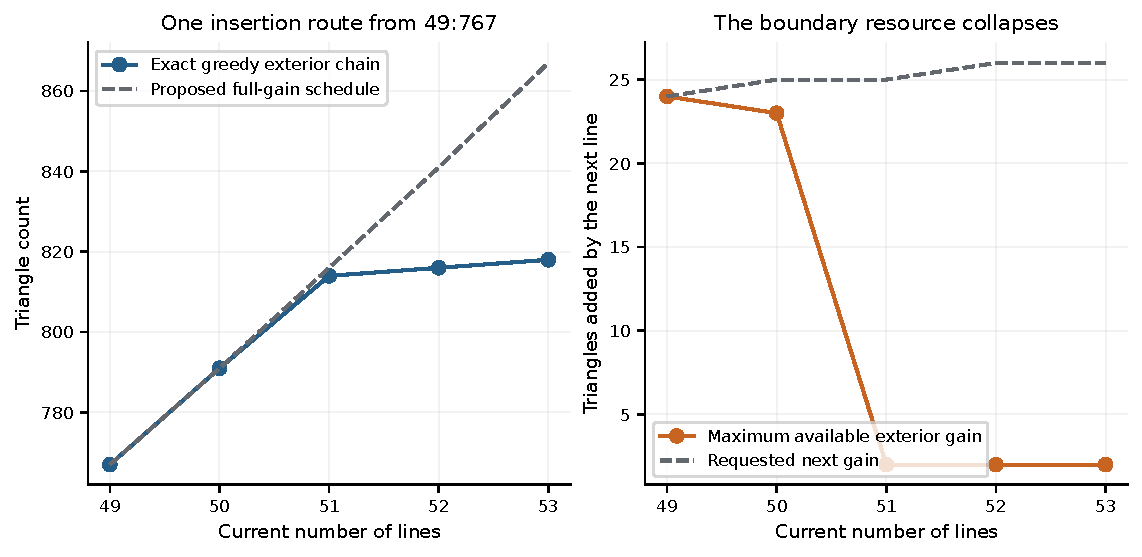
\includegraphics[width=0.88\linewidth]{figures/successor-49-resource.pdf}
\caption{The boundary resource in the particular exact 49-line chain.
The sharp drop in available wedges explains why its first full-gain
extension cannot be repeated with the requested next gain.  The plotted
capacities concern this chain only.}
\label{fig:successor}
\end{figure}

\subsection{A conditional recurrence and an unconditional numerical bound}

For any integer-valued function $F$, assume
\begin{equation}
 F(n+1)\geq F(n)+\lfloor n/2\rfloor\qquad(n\geq s).
 \label{ext:full-step}
\end{equation}
Summation, including both parity cases, gives the fully checked arithmetic
implication
\begin{equation}
 F(n)\geq F(s)+
 \left\lfloor\frac{(n-1)^2}{4}\right\rfloor-
 \left\lfloor\frac{(s-1)^2}{4}\right\rfloor
 \qquad(n\geq s).
 \label{ext:conditional-closed}
\end{equation}
The hypothesis \eqref{ext:full-step} remains explicit in the formal
theorem.  Substituting $s=49$ and $F(49)=767$ yields the numerical target
\begin{equation}
 Q_{49}(n)=\left\lfloor\frac{(n-1)^2}{4}\right\rfloor+191.
 \label{ext:49-target}
\end{equation}

There is now a separate unconditional Lean theorem
\begin{equation}
 \K(n)\geq Q_{49}(n)\qquad(n\geq49),
 \label{ext:49-unconditional}
\end{equation}
proved using the saved witnesses at 49 and 50 and the classical all-order
baseline thereafter.  Indeed, for $n\geq51$,
\[
 \frac{n(n-3)}3-\frac{(n-1)^2}4-191
 =\frac{n^2-6n-2295}{12}\geq0,
\]
with equality at $n=51$ and an increasing numerator beyond it.  Rounding
gives $\B(n)\geq Q_{49}(n)$.  This proves the desired numerical formula
without constructing a nested full-gain chain.  The stronger all-order
bound $\G$ and the finite envelope elsewhere in this paper also dominate
it.

For comparison, direct iteration of the defect rule
$T_{n+1}=T_n+g(n,T_n)$ from $49:767$ guarantees
$50:791$, $51:803$, $52:805$, and $60:821$.
The stronger target \eqref{ext:49-target} gives $51:816$, $52:841$, and
$60:1061$.  These are different constructions and different assertions.
The completed numerical theorem does not retrospectively prove the
March extension claim, and the failure of its proposed exterior
iteration does not invalidate the completed numerical theorem.
